\subsubsection{Guidance method's questionnaire.}
\label{subsubsec:results_questionnaires_2}

As for the blind users, the sighted user also answered the Guidance questionnaire to give their thoughts about their experience with the guidance methods. Table \ref{tab:questionnaire_average} shows the score of both groups. The corresponding barplots are presented in Figure \ref{fig:barplot_questionnaire_scene_blind_sight}. Both groups prefer audio  and mixture methods. The difference lies in the preference between the haptic belt and virtual cane. The blind users tend to prefer the first one, while the sighted users tend to prefer the last.


\begin{table}[!htb]
\centering
\caption{Guidance method questionnaire average score grouped by participant.}
\label{tab:questionnaire_average}
\begin{tabular}{lllrrrrr}
\toprule
{} & Audio & \begin{tabular}[c]{@{}l@{}}Haptic\\ Belt\end{tabular} & \begin{tabular}[c]{@{}l@{}}Virtual\\ Cane\end{tabular} & Mixture & Visual Condition \\
Participant &       &                                                       &                                                        &         &                  \\
\midrule
001         &  0.75 &                                                  0.49 &                                                   0.57 &    0.69 &            Sight \\
001C        &  0.77 &                                                  0.54 &                                                   0.63 &    0.87 &            Blind \\
002C        &  0.86 &                                                  0.74 &                                                   0.54 &    0.93 &            Blind \\
003         &  0.76 &                                                  0.54 &                                                   0.54 &    0.78 &            Sight \\
003C        &  0.93 &                                                  0.57 &                                                   0.54 &    0.74 &            Blind \\
004         &  0.86 &                                                  0.60 &                                                   0.79 &    0.76 &            Sight \\
004C        &  0.88 &                                                  0.49 &                                                   0.40 &    0.73 &            Blind \\
005         &  0.61 &                                                  0.57 &                                                   0.75 &    0.84 &            Sight \\
\bottomrule
\end{tabular}
\end{table}



\begin{figure}[!htb]
    \centering
    \begin{minipage}{\textwidth}
        \centering
        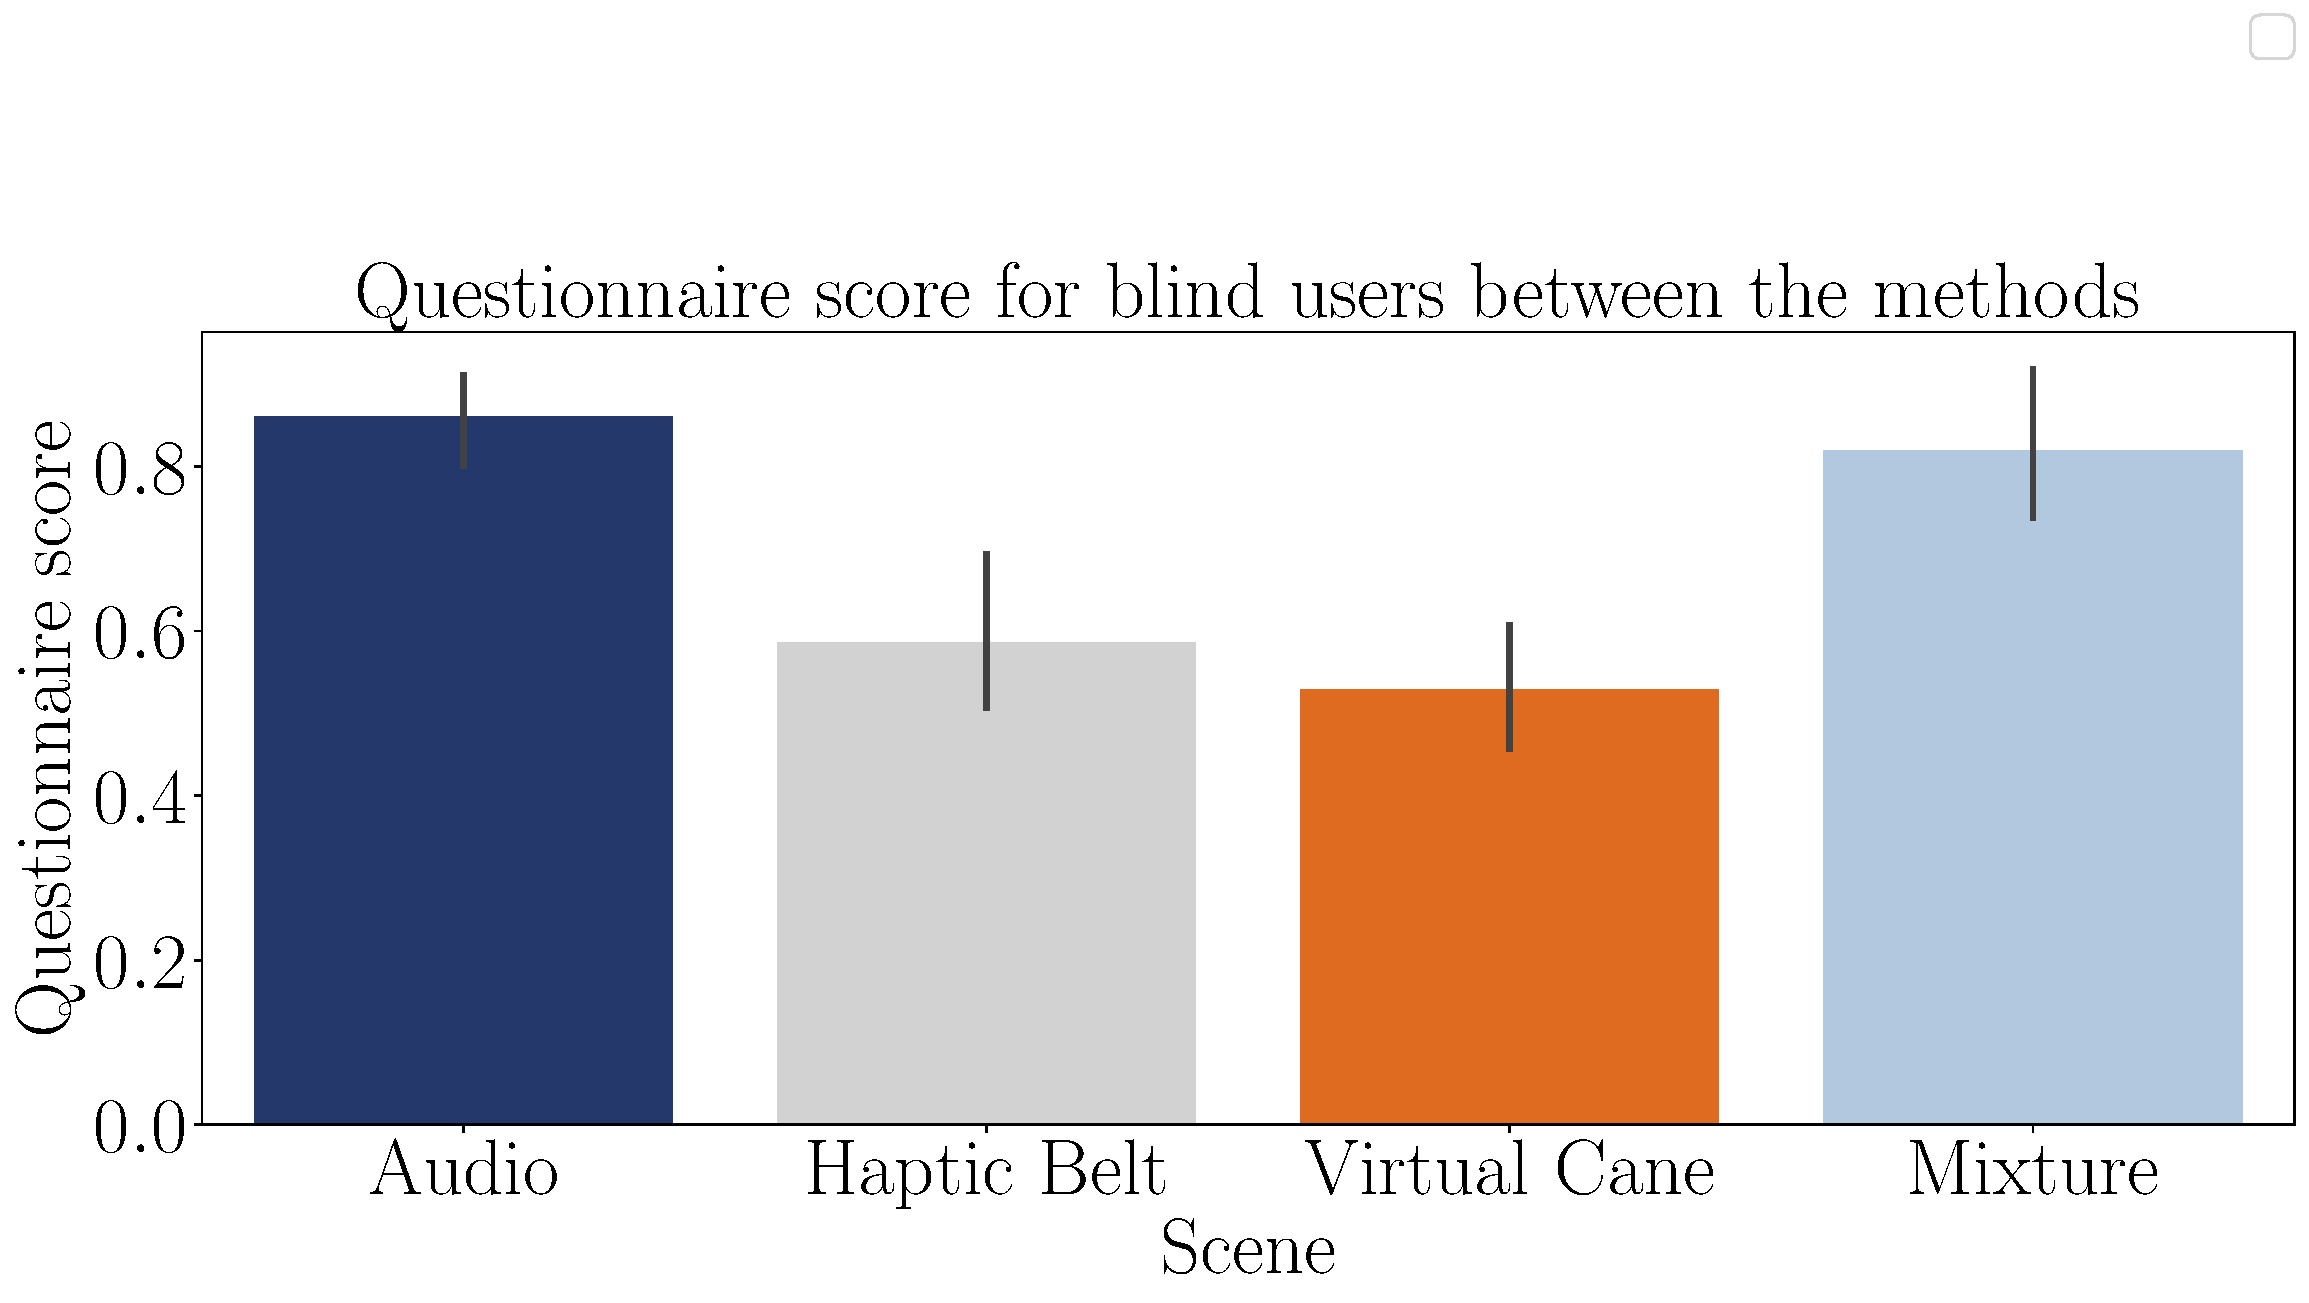
\includegraphics[width = \textwidth]{Resultados/Questionario/Figuras/pdf/barplot_questionnaire_scene_blind.pdf}
        \subcaption{Blind participants.}
        \label{fig:barplot_questionnaire_scene_blind_2}
    \end{minipage}
    \begin{minipage}{\textwidth}
        \centering
        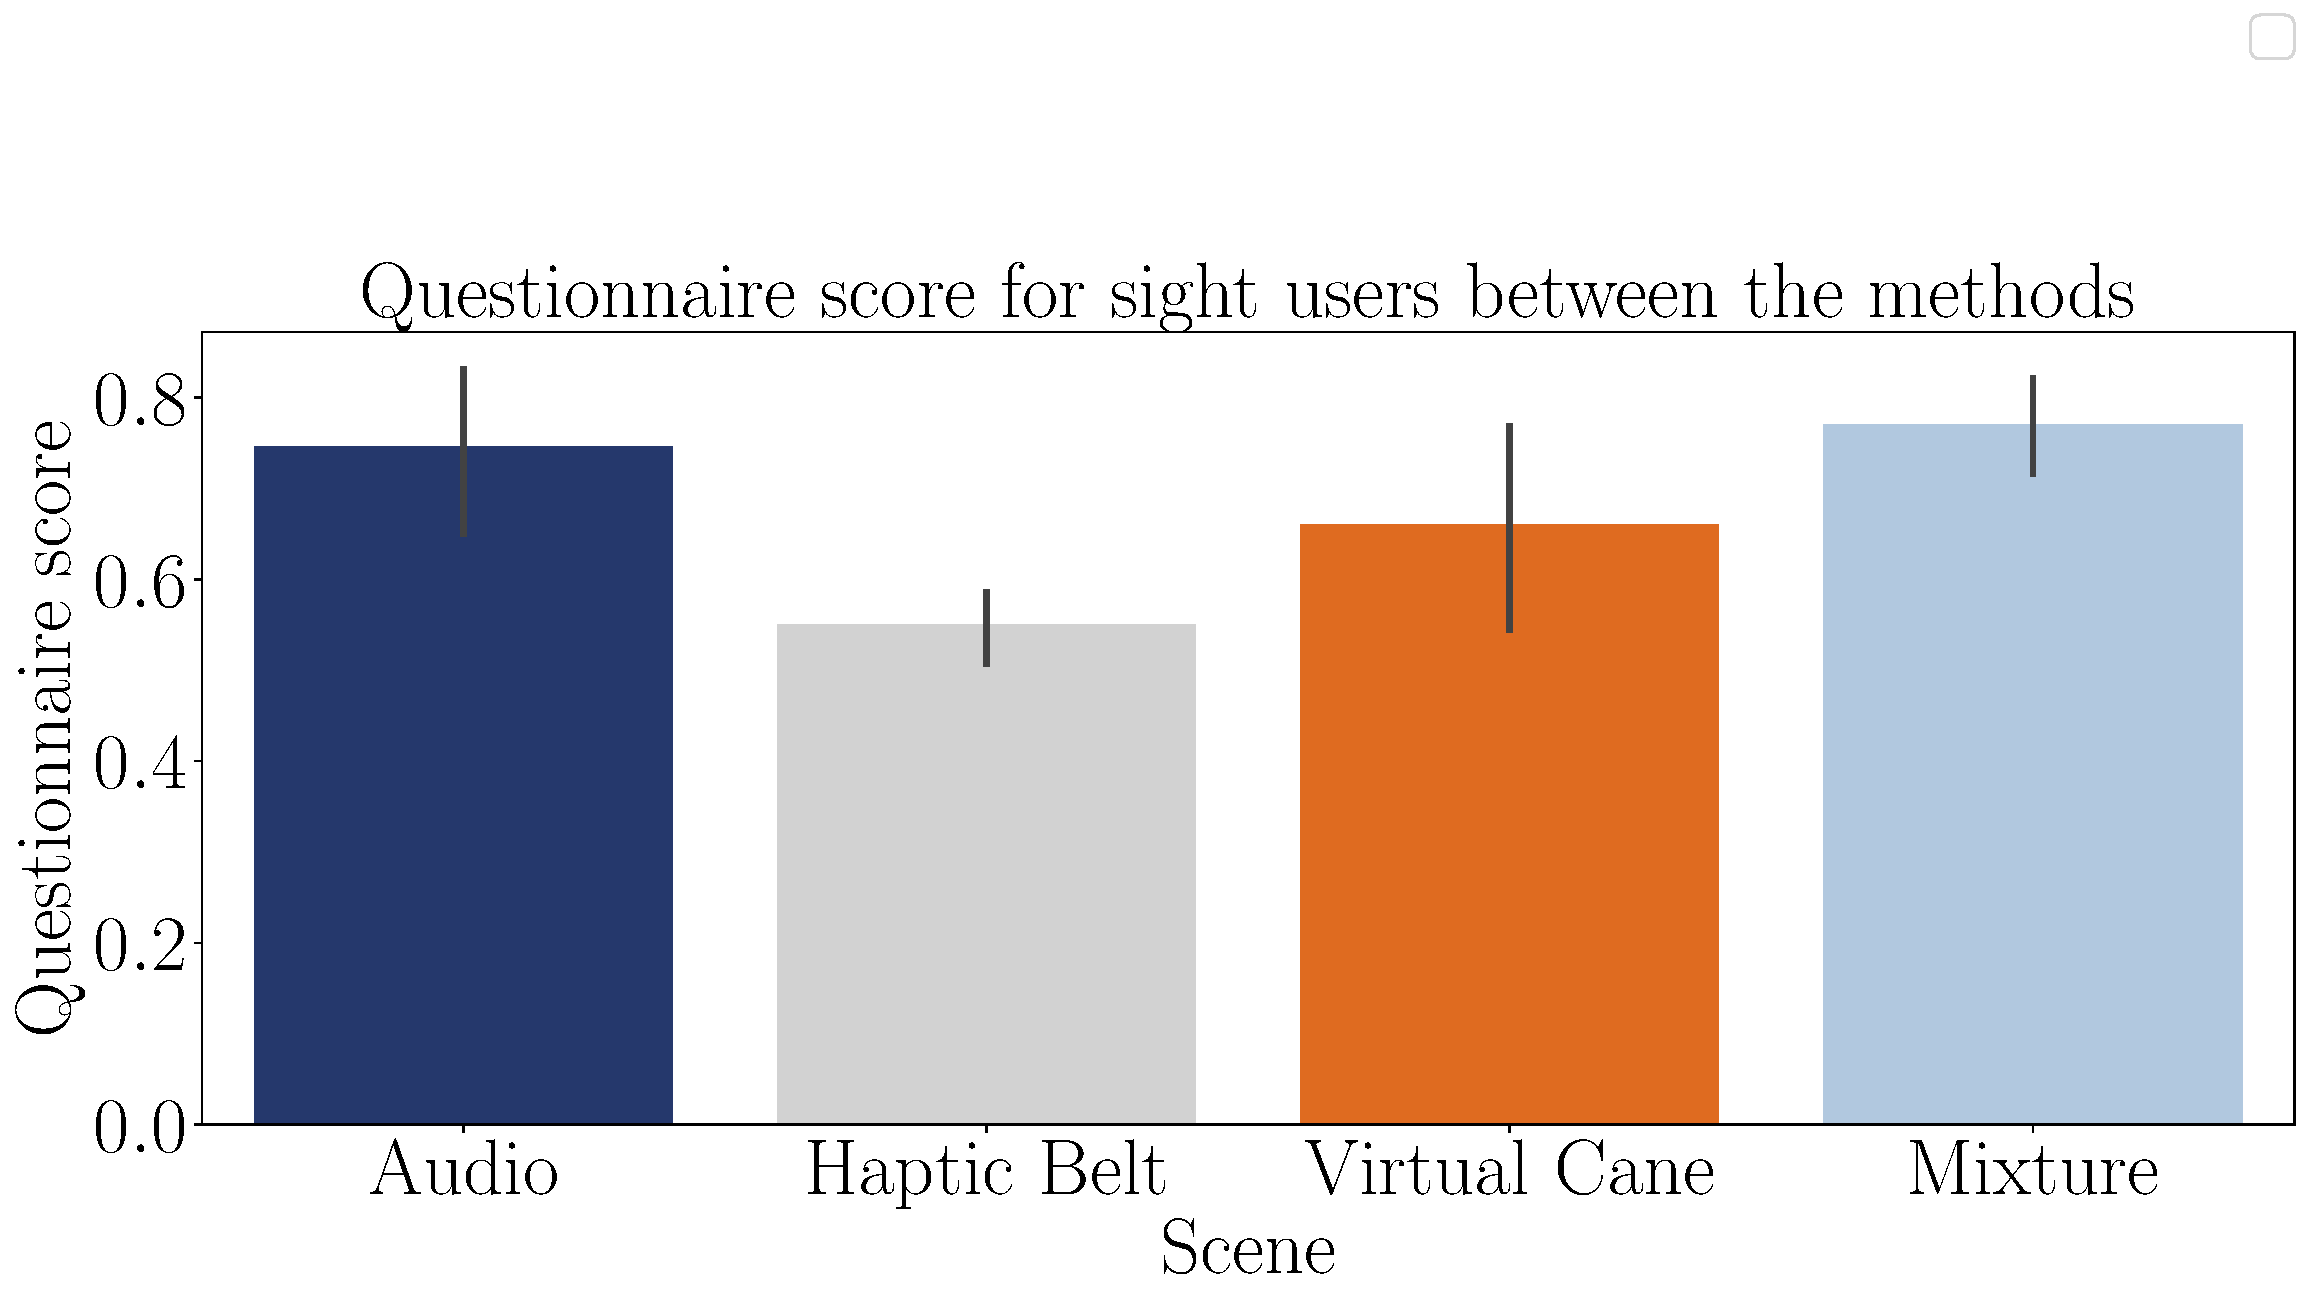
\includegraphics[width = \textwidth]{Resultados/Questionario/Figuras/pdf/barplot_questionnaire_scene_sight.pdf}
        \subcaption{Sighted participants.}
        \label{fig:barplot_questionnaire_scene_sight}
    \end{minipage}
    \caption{Barplot of the average questionaire score on each method.}
    \label{fig:barplot_questionnaire_scene_blind_sight}
\end{figure}
%\begin{figure}[!htb]
%    \centering
%    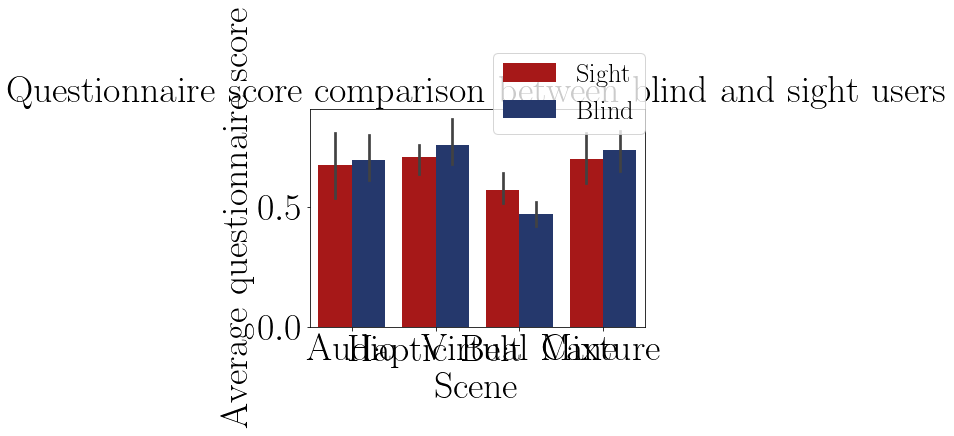
\includegraphics[width = \textwidth]{Resultados/Questionario/Figuras/png/barplot_questionnaire_scene.png}
%    \caption{Barplot of the  average questionaire score of both participants on each method.}
%    \label{fig:barplot_questionnaire_scene}
%\end{figure}

The Figure \ref{fig:boxplot_questionnaire_scene} presents the box plot with the distribution of the scores. It is possible to see that there is some similarity between the two groups, except for the virtual cane method, which has a broader distribution for the sighted users. Also, it seems that the audio and mixture have similar acceptance for sighted and blind users.

\begin{figure}[!htb]
    \centering
    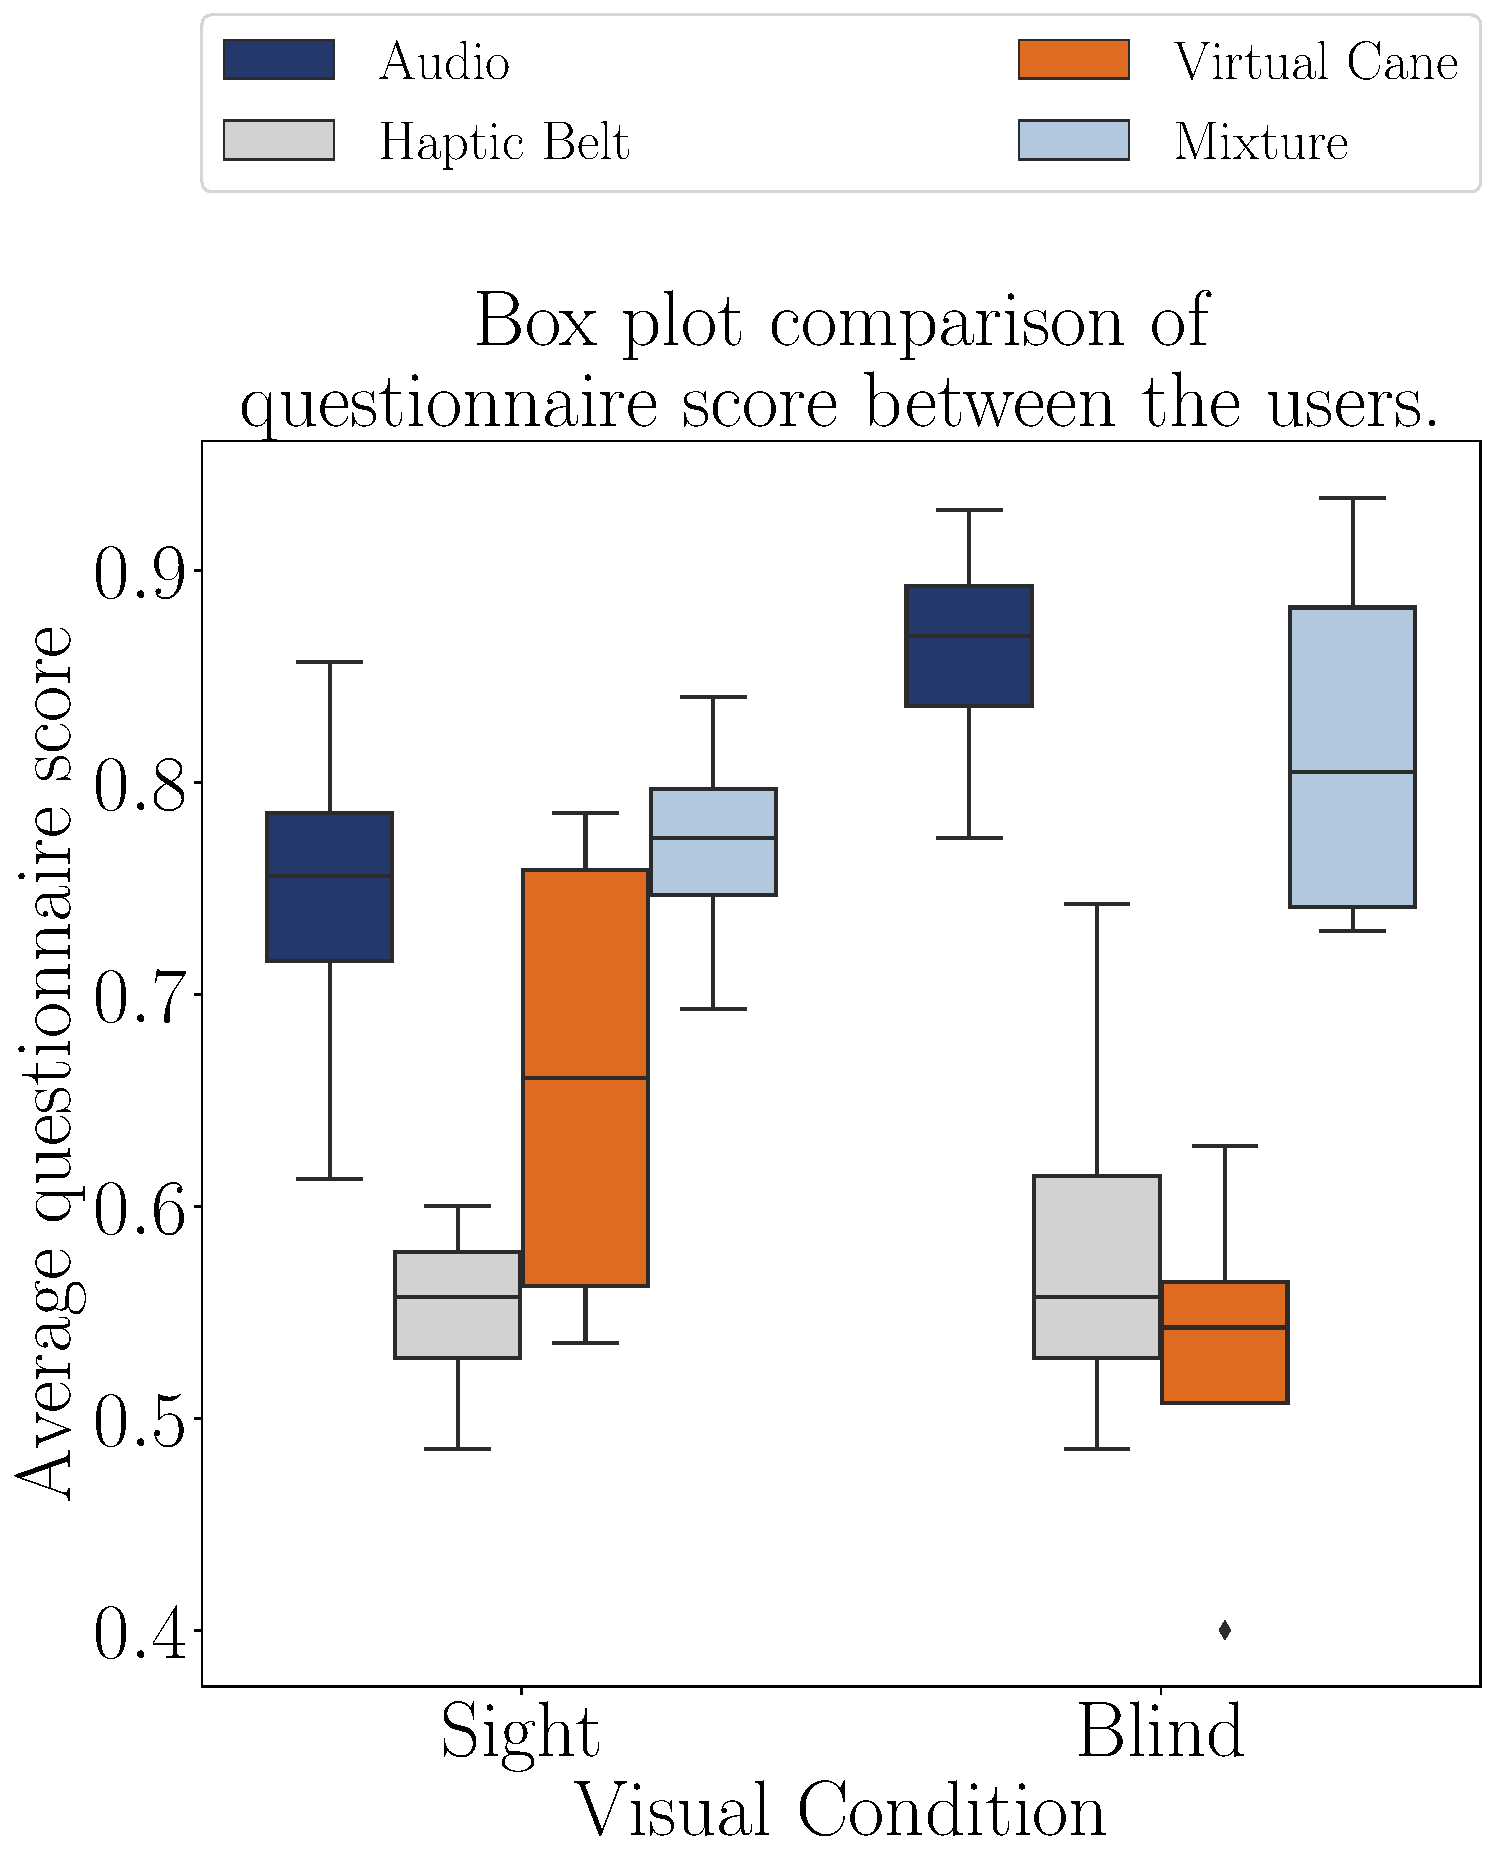
\includegraphics[width = 0.45\textwidth]{Resultados/Questionario/Figuras/pdf/boxplot_questionnaire_scene.pdf}
    \caption{Boxplot of the questionaire score of the the participants grouped by the methods.}
    \label{fig:boxplot_questionnaire_scene}
\end{figure}

%The Table \ref{tab:questionnaire_average_group} show the the average questionnaire score on each method of both groups and it shows the same conclusion as the Figure \ref{fig:barplot_questionnaire_scene}, that the preference between the "Haptic Belt" and "Virtual Cane" is the only difference between the two groups.
%
%Considering the most preferable and the less preferable of each group, the blind users are score their choices more intesiver than the sighted users. This may be an effect from their previous experience with the "Audio" method in previous events before the experiment and with haptic devices were something very, or almost, new. For the sighted users everything was new, so there scores were more consistent. This is posible to see in the average and standar deviation of these scores. For the blind users is 0.7 and 0.164 and for the sighted user is 0.682 and 0.100.
%
%
\begin{table}[!htb]
\centering
\caption{Guidance method questionnaire average score grouped by visual condition.}
\label{tab:questionnaire_average_group}
\begin{tabular}{lllll}
\toprule
{} &  Audio &  Haptic Belt &  Virtual Cane &  Mixture \\
Visual Condition &        &              &               &          \\
\midrule
Blind            &  0.693 &        0.757 &         0.471 &    0.735 \\
Sight            &  0.674 &        0.707 &         0.571 &    0.698 \\
\bottomrule
\end{tabular}
\end{table}



Figures \ref{fig:qqplot_questionnaire_sight} and \ref{fig:residplot_questionnaire_sight} brings the QQ plot and residual distribution, which confirm that ANOVA can be applied. The result of ANOVA is presented in Table \ref{tab:blocanova_questionnaire_blind_sight} and indicates that the method is an effective variable for the sighted participants, as it is for the blind ones.

\begin{table}[!htb]
    \caption{Anova p-value for the questionnaire score on each method}
    \label{tab:blocanova_questionnaire_blind_sight}
\begin{minipage}{0.45\textwidth}
    \subcaption{Blind participants.}
    
\centering
\begin{tabular}{ll}
\toprule
Source & P-Value \\
\midrule
Method & 0.001** \\
\bottomrule
\end{tabular}

\end{minipage}
\begin{minipage}{0.45\textwidth}
    \subcaption{Sight participants.}
    
\centering
\begin{tabular}{ll}
\toprule
Source & P-Value \\
\midrule
Method & 0.016** \\
\bottomrule
\end{tabular}

\end{minipage}
\end{table}

\begin{figure}[!htb]
    \centering
    %\vspace{-15.0cm}
    \begin{minipage}{0.45\textwidth}
        \centering
        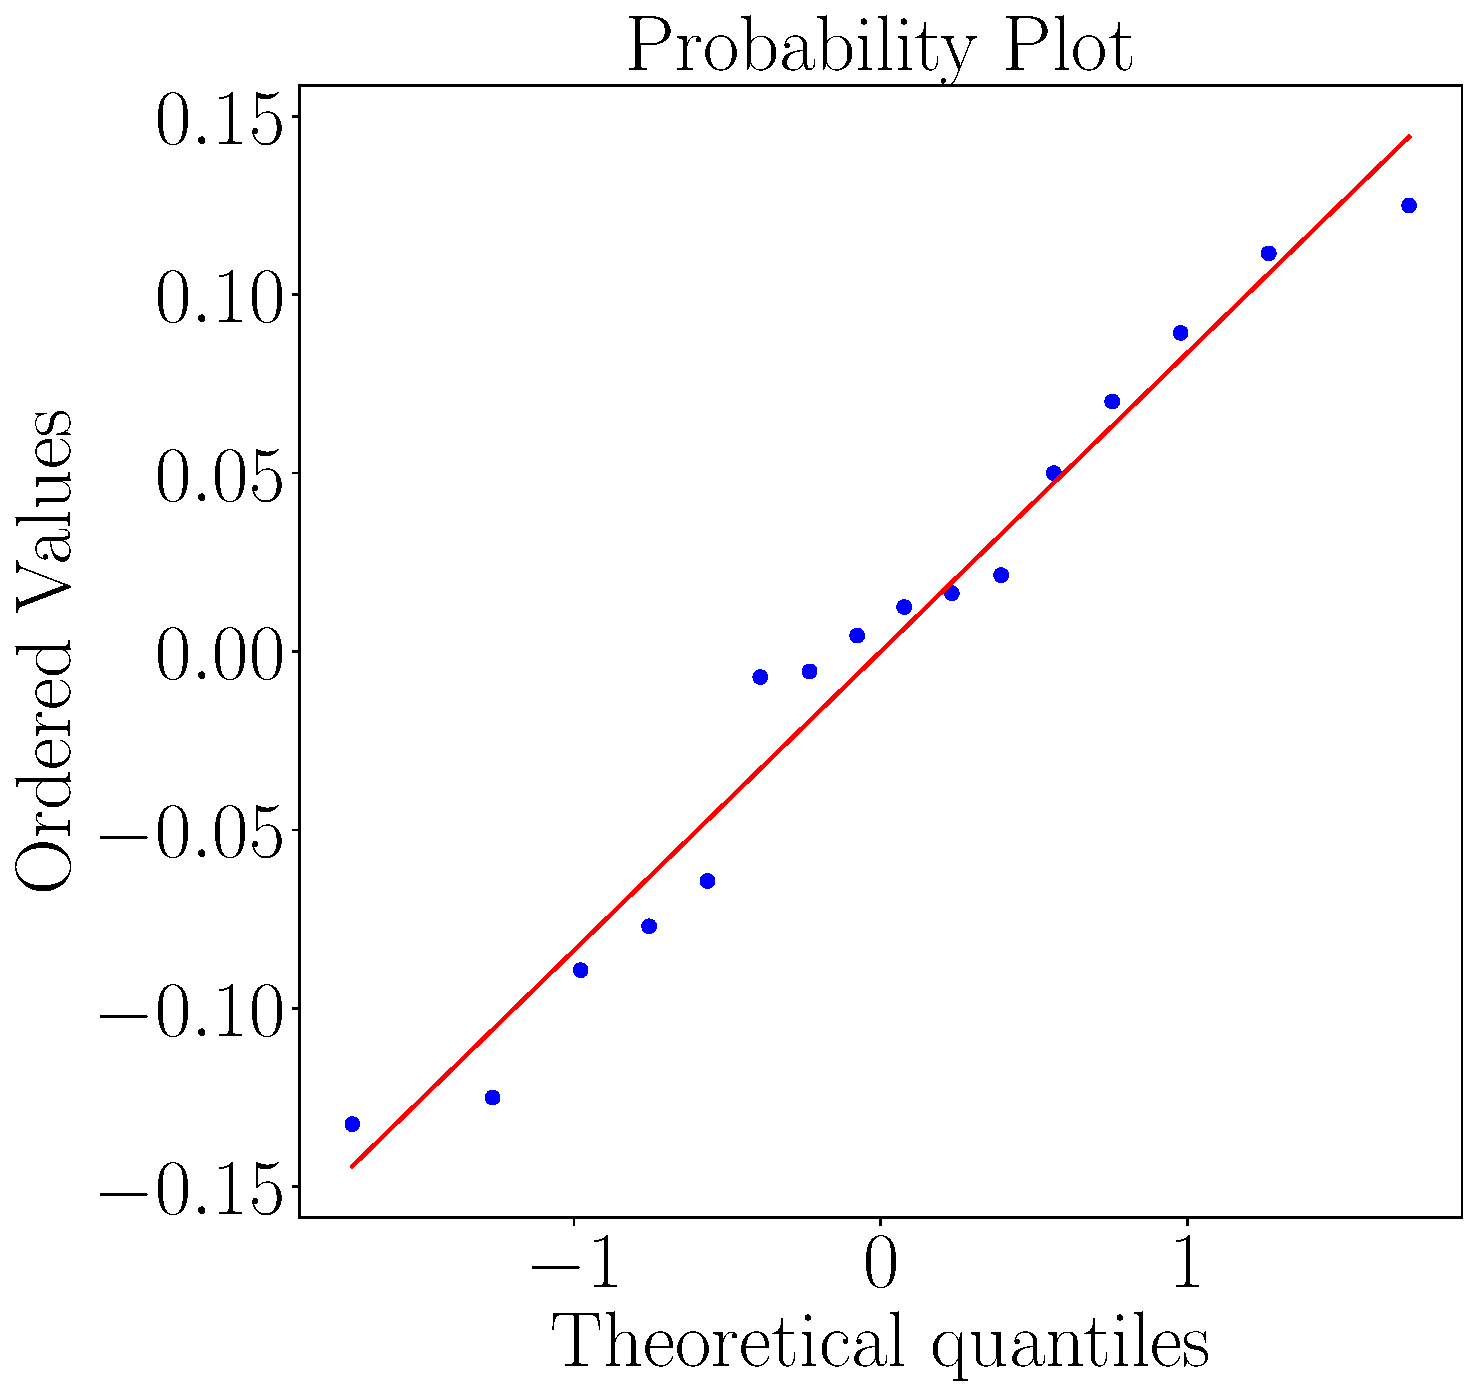
\includegraphics[width = \textwidth]{Resultados/Questionario/Figuras/pdf/qqplot_questionnaire_sight.pdf}
        \caption{QQ plot of the questionnaire score of the sighted participants on each method.}
        \label{fig:qqplot_questionnaire_sight}
    \end{minipage}
    \begin{minipage}{0.075\textwidth}
        \hfill
    \end{minipage}
    \begin{minipage}{0.45\textwidth}
        \centering
        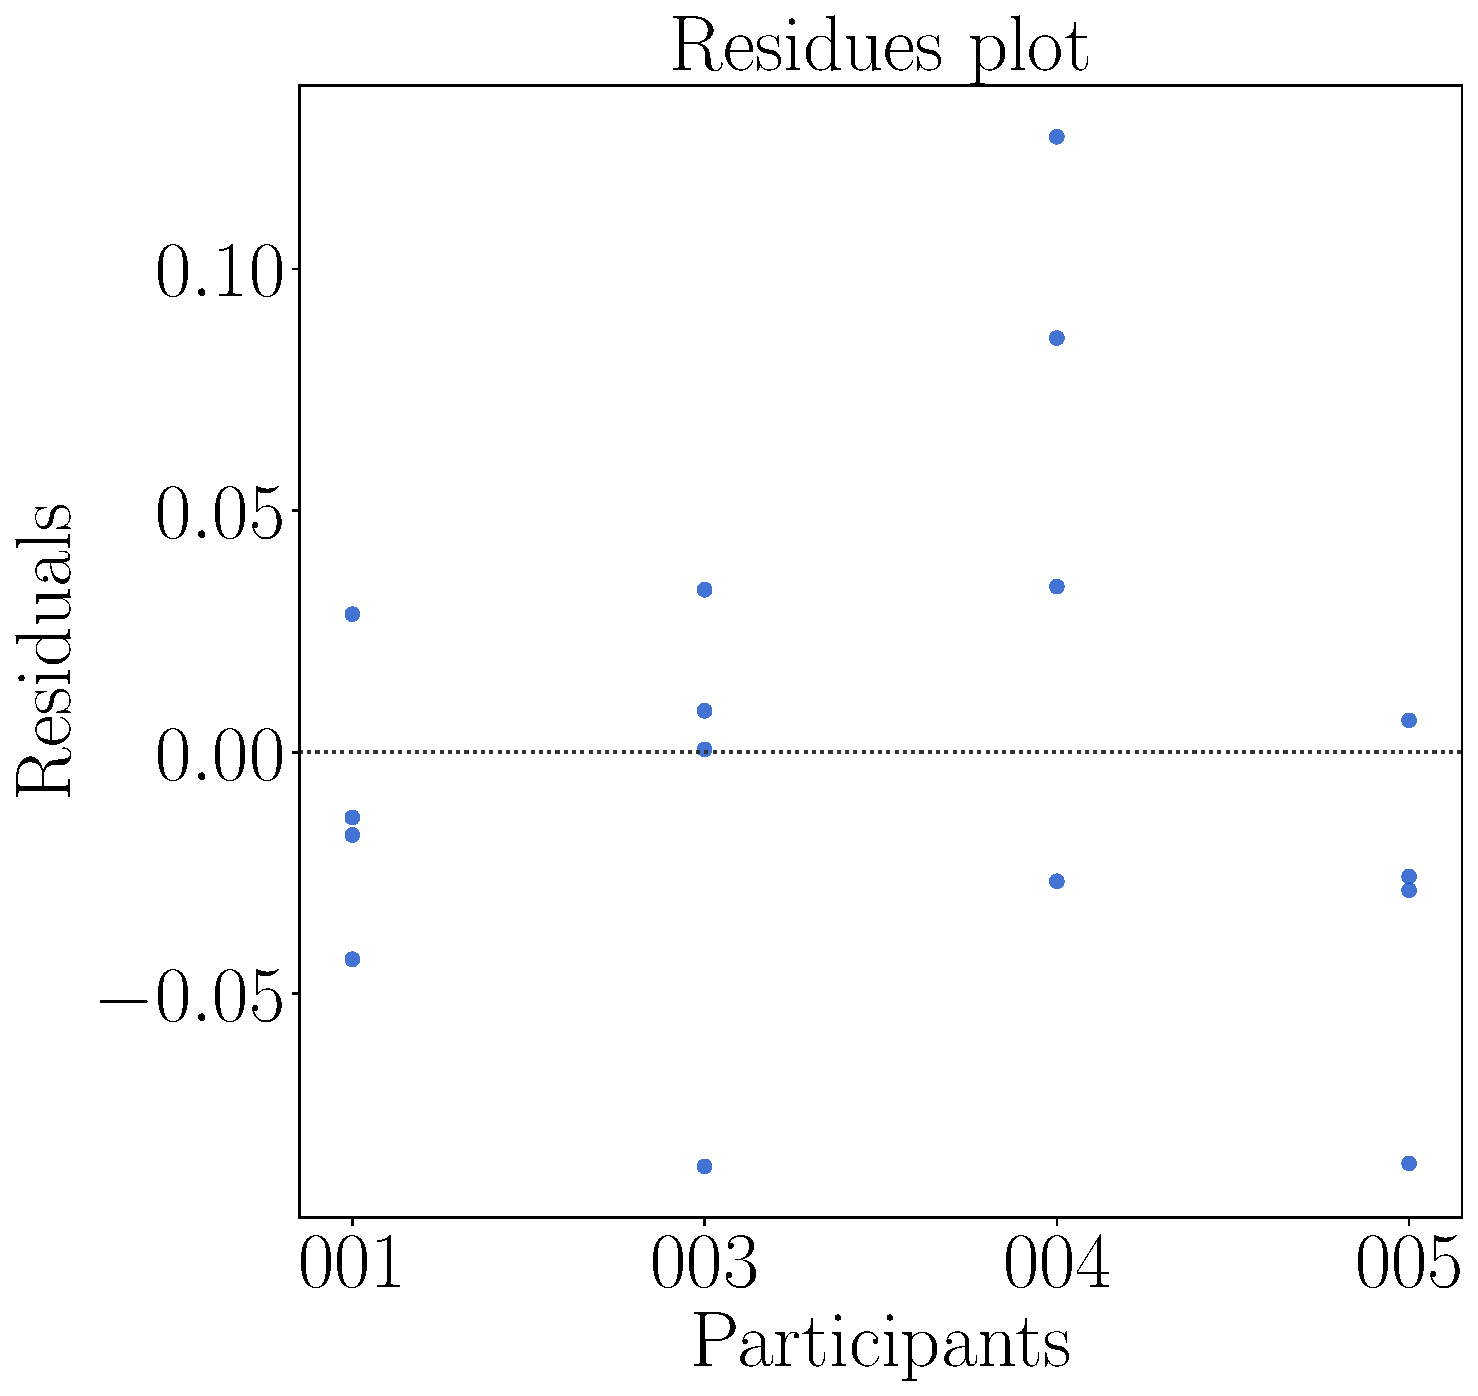
\includegraphics[width = \textwidth]{Resultados/Questionario/Figuras/pdf/residplot_questionnaire_sight.pdf}
        \caption{Residual plot of the questionnaire score the sighted participants on each method.}
        \label{fig:residplot_questionnaire_sight}
    \end{minipage}
\end{figure}

Table \ref{tab:lsd_questionnaire_blind_sight} presents the conclusion of a pairwise Fisher LSD test between all the guidance methods for both groups, showing that the results are coincident.

\FloatBarrier

\begin{table}[!thb]
    \caption{Anova p-value for the mental demand average on each method'}
    \label{tab:lsd_questionnaire_blind_sight}
    \begin{minipage}{1\textwidth}
        \subcaption{Blind participants.}
        
\centering
\begin{tabular}{rclr}
\toprule
      \multicolumn{3}{c}{Method} &                                           Analysis \\
\midrule
       Audio & $X$ & Haptic Belt &        $H_1 : \mu_{Audio} \ne \mu_{Haptic Belt}**$ \\
      Audio & $X$ & Virtual Cane &       $H_1 : \mu_{Audio} \ne \mu_{Virtual Cane}**$ \\
           Audio & $X$ & Mixture &                $H_0 : \mu_{Audio} = \mu_{Mixture}$ \\
Haptic Belt & $X$ & Virtual Cane & $H_1 : \mu_{Haptic Belt} \ne \mu_{Virtual Cane}**$ \\
     Haptic Belt & $X$ & Mixture &      $H_1 : \mu_{Haptic Belt} \ne \mu_{Mixture}**$ \\
    Virtual Cane & $X$ & Mixture &     $H_1 : \mu_{Virtual Cane} \ne \mu_{Mixture}**$ \\
\bottomrule
\end{tabular}

    \end{minipage}
    \begin{minipage}{1\textwidth}
        \subcaption{Sight participants.}
        
\centering
\begin{tabular}{rclr}
\toprule
      \multicolumn{3}{c}{Method} &                                           Analysis \\
\midrule
       Audio & $X$ & Haptic Belt &        $H_1 : \mu_{Audio} \ne \mu_{Haptic Belt}**$ \\
      Audio & $X$ & Virtual Cane &       $H_1 : \mu_{Audio} \ne \mu_{Virtual Cane}**$ \\
           Audio & $X$ & Mixture &                $H_0 : \mu_{Audio} = \mu_{Mixture}$ \\
Haptic Belt & $X$ & Virtual Cane & $H_1 : \mu_{Haptic Belt} \ne \mu_{Virtual Cane}**$ \\
     Haptic Belt & $X$ & Mixture &      $H_1 : \mu_{Haptic Belt} \ne \mu_{Mixture}**$ \\
    Virtual Cane & $X$ & Mixture &     $H_1 : \mu_{Virtual Cane} \ne \mu_{Mixture}**$ \\
\bottomrule
\end{tabular}

    \end{minipage}
\end{table}

%
\begin{table}[!htb]
\centering
\caption{Cross validation p-value for the questionnaire score on each method for blinded users.}
\label{tab:lsd_questionnaire}
\begin{tabular}{rclr}
\toprule
      \multicolumn{3}{c}{Method} &                                           Analysis \\
\midrule
       Audio & $X$ & Haptic Belt &        $H_1 : \mu_{Audio} \ne \mu_{Haptic Belt}**$ \\
      Audio & $X$ & Virtual Cane &       $H_1 : \mu_{Audio} \ne \mu_{Virtual Cane}**$ \\
           Audio & $X$ & Mixture &                $H_0 : \mu_{Audio} = \mu_{Mixture}$ \\
Haptic Belt & $X$ & Virtual Cane & $H_1 : \mu_{Haptic Belt} \ne \mu_{Virtual Cane}**$ \\
     Haptic Belt & $X$ & Mixture &          $H_0 : \mu_{Haptic Belt} = \mu_{Mixture}$ \\
    Virtual Cane & $X$ & Mixture &     $H_1 : \mu_{Virtual Cane} \ne \mu_{Mixture}**$ \\
\bottomrule
\end{tabular}
\end{table}



%The LSD Table \ref{tab:lsd_questionnaire_sight} repeat the same conclusion of the blind participants, that only the "Audio" and "Mixture" are statistically the same. But that does not mean that both groups had the same opinion from the rest of the methods. As shown in the Figure \ref{fig:boxplot_questionnaire_scene}, the average sighted user rather use the "Virtual Cane" then the "Haptic Belt", despite that distribution being wider, hence more varied, meaning that this is hardly a consense between the users.

%\FloatBarrier